\documentclass{beamer}

\usepackage{txfonts}
\usepackage{hyperref}
\usepackage{fancybox}
\usepackage{xfrac}
\usepackage{cancel,slashbox}

\newcommand{\heart}{\ensuremath\heartsuit}

\usepackage{mathtools,amssymb}
\newcommand{\myarrow}{\scalebox{2}[2]{$\mathclap{\curvearrowleft}\mkern2.2mu
                                                 \mathclap{\curvearrowright}$}}

\DeclareMathOperator{\Bin}{\mathrm{Bin}}
\DeclareMathOperator{\Max}{\mathrm{Max}}

\hypersetup{colorlinks=false,linkbordercolor=red,linkcolor=green,pdfborderstyle={/S/U/W 1}}

\addtobeamertemplate{navigation symbols}{}{ \hspace{1em}    \usebeamerfont{footline}%
    \insertframenumber / \inserttotalframenumber}

\geometry{papersize={15cm,15cm}}
\usepackage{lipsum}

\makeatletter
\newenvironment<>{contdproof}[1][\proofname]{%
    \par
    \def\insertproofname{#1\@addpunct{.}}%
    \usebeamertemplate{proof begin}#2}
  {\usebeamertemplate{proof end}}
\makeatother


\setbeamertemplate{theorems}[numbered]

\newtheorem{remark}{Remark}



\newtheorem*{nonumdefinition}{Definition}
\newtheorem*{nonumproblem}{Problem}
\newtheorem*{nonumcorollary}{Corollary}
\newtheorem*{nonumlemma}{Lemma}
\newtheorem*{nonumproof}{Proof}
\newtheorem*{nonumtheorem}{Theorem}
\newtheorem*{nonumremark}{Remark}
\newtheorem*{answer}{Answer}
\newtheorem*{nonumremarks}{Remarks}
\newtheorem*{nonumexamples}{Examples}
\newtheorem*{nonumsolution}{Solution}
\newtheorem*{nonumexample}{Example}
\newtheorem*{nonumproposition}{Proposition}
\newtheorem{proposition}[theorem]{Proposition}

\usepackage{tikz}
\newcommand*\mycirc[1]{%
  \tikz[baseline=(C.base)]\node[draw,circle,inner sep=.7pt](C) {#1};\:
}

\newcommand\myheading[1]{%
  \par\bigskip
  {\color{blue}{\large #1}}\par\smallskip}

%\usetheme{Warsaw}
%\usetheme{Berkeley} %sample 1

\usetheme{Berlin} % sample 2
%\usetheme{AnnArbor} % sample 3

\let\otp\titlepage
\renewcommand{\titlepage}{\otp\addtocounter{framenumber}{-1}}

\title{Lecture 16 : Independence, Covariance and Correlation of Discrete Random Variables}
\author{}
\date{}

\begin{document}
\begin{frame}[plain]
\titlepage
\end{frame}

\begin{frame}
\begin{nonumdefinition}
Two discrete random variables $X$ and $Y$ defined on the same sample space are said to be independent if for nay two numbers $x$ and $y$ the two events $(X=x)$ and $(Y=y)$ are independent $\Leftrightarrow$
\begin{equation*}
\text{
\includegraphics{figure/fig1.eps}}\tag{*}\label{eq-*}
\end{equation*}
\end{nonumdefinition}
\end{frame}

\begin{frame}
Now \eqref{eq-*} say the \underline{joint} $pmf$ $P_{X,Y}(x,y)$ is determined by the \underline{marginal} $pmf$'s $P_{X}(x)$ and $P_{Y}(y)$ by taking the product.

\begin{nonumproblem}
In case $X$ and $Y$ are independent how do you recover the matrix (table) representing $P_{X,y}(x,y)$ from its margins?
\end{nonumproblem}
\end{frame}

\begin{frame}
Let's examine the table for the standard example
\begin{center}
\renewcommand{\arraystretch}{1.2}
\begin{tabular}{c|c|c|c|c|c}
\backslashbox{$X$}{$Y$} & 0 & 1 & 2 & 3 & \\
\hline
0 & $\frac{1}{8}$ & $\frac{2}{8}$ & $\frac{1}{8}$ & 0 & $\frac{1}{2}$\\
\hline
1 & 0 & $\frac{1}{8}$ & $\frac{2}{8}$ & $\frac{1}{8}$ & $\frac{1}{2}$\\
\hline
 & $\frac{1}{8}$ & $\frac{3}{8}$ & $\frac{3}{8}$ & $\frac{1}{8}$ & 
\end{tabular}
\end{center}

Note that

\smallskip
\qquad $X = \sharp$ of heads on the first toss

\qquad $Y$ = total $\sharp$ of heads in all three tosses
\smallskip

So we wouldn't expect $X$ and $Y$ to be independent (if we know $X=1$ that restricts the values of $Y$.)
\end{frame}

\begin{frame}
Lets use the formula \eqref{eq-*}

It says the following.

Each position inside the table corresponds to two positions on the margins
\begin{enumerate}
\item Go to the right

\item Go Down

\smallskip
\centerline{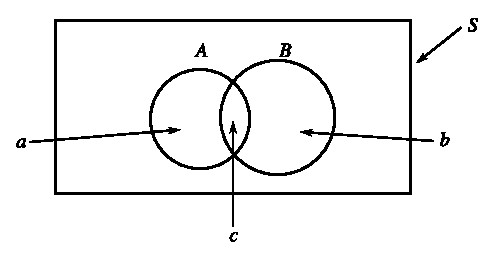
\includegraphics{figure/fig2.eps}}
\smallskip
\end{enumerate}

So in the picture
\begin{enumerate}
\item If we go right we get $\dfrac{1}{2}$

\item If we go down we get $\dfrac{3}{8}$
\end{enumerate}
\end{frame}

\begin{frame}
%raghu, page 5
\end{frame}

\begin{frame}

\end{frame}

\begin{frame}

\end{frame}

\begin{frame}

\end{frame}

\begin{frame}

\end{frame}

\begin{frame}

\end{frame}

\begin{frame}

\end{frame}

\begin{frame}

\end{frame}

\begin{frame}

\end{frame}

\begin{frame}

\end{frame}

\begin{frame}

\end{frame}

\begin{frame}

\end{frame}

\begin{frame}

\end{frame}

\begin{frame}

\end{frame}

\begin{frame}

\end{frame}

\begin{frame}

\end{frame}

\begin{frame}

\end{frame}

\begin{frame}

\end{frame}

\begin{frame}

\end{frame}

\begin{frame}

\end{frame}

\begin{frame}

\end{frame}

\begin{frame}

\end{frame}

\begin{frame}

\end{frame}

\begin{frame}

\end{frame}

\begin{frame}

\end{frame}

\begin{frame}

\end{frame}

\begin{frame}

\end{frame}

\end{document}


